\chapter{Materials \& Methods} \label{chapter:materials-methods}

% 학위 논문의 결과를 도출하는 데에 사용한 실험 재료와 방법을 타인이 반복 실험 시 동일한 결과를 얻을 수 있을 정도로 자세히 기술한다.
% 방법에 따라 다음과 같이 부제를 넣어 기술한다.

% 예)
% 2.1 식물 재료 및 생장 조건
% 2.2 뿌리 관속 조직 관찰
% 2.3 유전자 발현 분석

\section{Overview of Current \texttt{Petasearch} Algorithm} \label{section:overview-of-current-algorithm}

An overview of the current \texttt{Petasearch} algorithm is visualized in \autoref{fig:overview}.
The algorithm contains the following three stages:

\begin{enumerate}[leftmargin=*]
  \item \textbf{Pre-processing phase}:
        In this phase, we first convert the input \texttt{FASTA/Q} file into a compressed \texttt{Petasearch} sequence database format (described in \cref{section:protein_sequence_compression}), and then we use the k-mer extraction tool to create the target tables.
        For each database, two tables were created.
        The first one contains the unique k-mers, the second one contains the corresponding sequence ID in the database.
        Instead of storing the k-mers as strings, we first converted the k-mers their numeric representations, and then sorted them.
        To further decrease the required amount of storage, we implemented a diff-index to store only the difference between k-mers, which is compressed using a creative bit-squeezing technique (described in \cref{section:diff-index_compression}), resulting in mostly 2 bytes of memory instead of 8 bytes per k-mer.
  \item \textbf{Prefiltering phase}: In the second step, we first create a query table for the input query sequence or profile database, extract all the k-mers inside and generate similar k-mers using either BLOSUM \cite{henikoff1992amino} matrices or the profile substitution matrix.
        We then perform a linear read and comparison between the query and target k-mers to find all the double k-mer matches. Such linear reading of the database is friendly to the caching and prefetch infrastructure of modern CPUs and modern NVMe SSDs.
        To maximize the huge NVMe linear read throughput, we also exploit advanced Linux IO techniques (described in \cref{section:io-performance}).
        After the comparison finishes, we sort the result and remove all entries where we have fewer than two hits for a target sequence from one query sequence to reduce random hits.
  \item \textbf{Alignment phase}: In the alignment phase, we read in the prefiltered results and retrieve the corresponding target sequence for the hits. In order to reduce unnecessary computation, we calculate the diagonal where the k-mer match occurred, which is the position of the k-mer in the target-sequence minus that in the query sequence.
  We skip the calculation if we do not find two diagonals within a distance of 4. Afterwards, we calculate the gapless alignment score for the all the diagonals and use the highest-scoring diagonal to compute SIMD-accelerated banded Smith-Waterman alignments.
\end{enumerate}

The contributions of the author were detailed in \cref{section:space-optimization}, \cref{section:speed-optimization} and \cref{section:sensitivity-improvement}.

\begin{figpage}
  \begin{figure}
    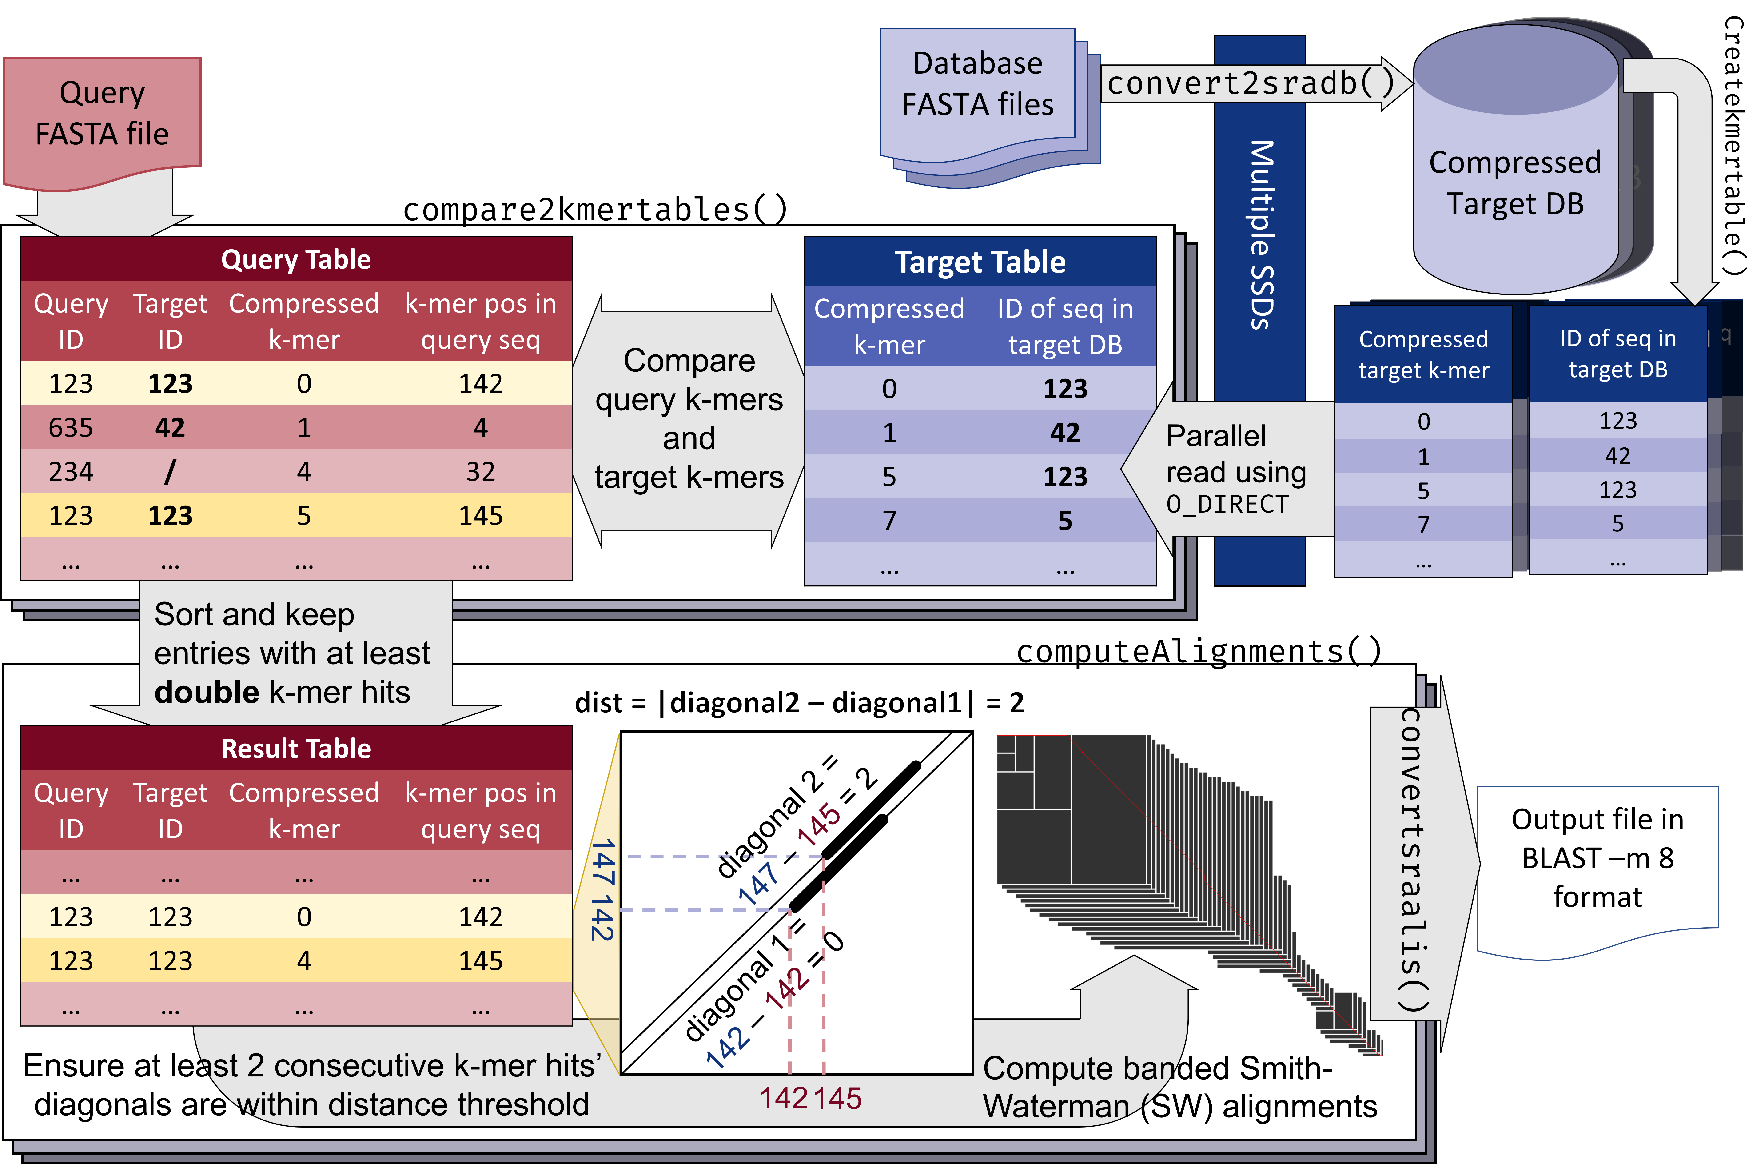
\includegraphics[width=\textwidth]{images/overview.pdf}
    \caption{
      \textbf{General overview of the Petasearch steps.} The preparation step, which will utilize the \texttt{convert2sradb()} and \texttt{createkmertable()} functions, creates the target tables that store all unique k-mers for each database. The pre-filtering step, which is implemented in \texttt{compare2kmertables()} consists of a highly parallelized double index search that streams the target tables directly from different solid state devices (SSDs) to saturate their maximum possible read rates and avoid random memory accesses. Requiring duplicate k-mer matches for each query-target sequence pair reduces the possibility of random hits and increases the specificity of the hits. An alignment for a query-target sequence pair is computed if the distance between diagonals for at least one k-mer pair is less than four. This constraint removes sequence pairs where the positions of the matching k-mers are not close and therefore a good alignment is unlikely. The alignment phase is realized in function \texttt{computeAlignment()} and the alignment output is possible to be converted into popular output formats such as the \texttt{BLAST -m 8} format.
    }
    \label{fig:overview}
  \end{figure}
\end{figpage}

\section{Space Optimization} \label{section:space-optimization}

The core idea of \texttt{Petasearch} is actually sacrificing space for fast computation.
However, the resources are not limitless.
Thus, we would like to keep the cost of space as low as possible while keeping the searching speed high.
In this section, we will discuss the space optimization techniques utilized to improve \texttt{Petasearch} prototype.

\subsection{Petasearch Data Structures Compression} \label{section:diff-index_compression}

As is described in \cref{section:overview-of-current-algorithm}, the values in diff-index created in the k-mer extraction step are usually able to fit inside a \texttt{short} integer.
However, when the difference is larger than \texttt{USHRT\_MAX}, in the prototypical implementation, we will store multiple \texttt{USHRT\_MAX} as long as the difference is larger than \texttt{USHRT\_MAX}.
This will make any k-mer difference larger than $4 \times \mathtt{USHRT\_MAX} = 262140$ require a larger space to store than the original \texttt{unsigned long} representation.
This situation is not uncommon especially when $k$ is large.

Also, in the prototypical implementation, the ID of the source sequence will also be stored multiple times in the ID table.
This redundancy is both unnecessary and troublesome.
It will increase the size of \texttt{Petasearch} data structures even more than the repeated \texttt{USHRT\_MAX} since the IDs are stored as \texttt{unsigned int} (32-bit integers).

\autoref{fig:k11_space} showed the space consumption of the diff-index created in the k-mer extraction step when $k = 11$.
Without optimization, the diff-index (k-mer table) and its corresponding ID table will take up 17 GB of space for a merely 1GB-sized database.

To optimize the size of the diff-index, we devised the bit-squeezing technique to compress the difference between two adjacent k-mers:
For any 64-bit k-mer difference, we continuously fetch 15 bits into a write buffer starting from the least significant bits.
We stop the retrieval until we encounter a zero chunk (15 bits of zeros).

To enable the correct decoding of the diff-index during the next phase, the sign bit of the last element in th write is set to \texttt{1} to indicate the end of encoding.
Afterwards, we write all the elements in the write buffer to the diff-index.
An example encoding process for difference of value $2039432531946$ is shown in \autoref{fig:bit_squeeze_technique}.
For ID table, the optimization is simple: we store the ID of the source sequence only once instead of repeatedly.

Using the bit-squeezing method, it is possible to obtain a maximum of five chunks, making the final space consumption larger than the size of a \texttt{unsigned long} integer.
However, such situation only happens when the difference is larger than $\texttt{1UL << 59} = 576460752303423488$, which is extremely rare.

While decoding the compressed diff-index in the process of double-index search, we will reverse the bit-squeezing process through repeatedly retrieving 15 bits from the diff-index table until we encounter the chunk with the sign bit set to \texttt{1}.
The decoded difference value will be add to the current k-mer.
Moreover, since we do not store redundant IDs, the ID pointer will not be incremented until the end of k-mer decoding.
\cref{algorithm:decode_kmer} showed the simplified pseudocode for k-mer decoding.

\begin{algorithm}[htbp]
  \begin{algorithmic}
    % \State $k = 11$
    \Procedure {DecodeKmer}{$currKmer$, $currTargetKmerPtr$, $currTargetIDPtr$}
    \State $currDiffIndex \gets 0$
    % \State $X \gets x$
    % \State$ $N \gets n$
    \While{\space$*currTargetKmerPtr > 0 $\space} \Comment{This means the sign bit is not 1.
    }
    \State $currDiffIndex \gets\ \textsc{Get15Bits}(*currTargetKmerPtr)$
    \State $currDiffIndex \gets currDiffIndex \texttt{ << } 15$
    \State $\textsc{Next}(currTargetKmerPtr)$
    \EndWhile
    \State $currDiffIndex \gets\ \textsc{Get15Bits}(*currTargetKmerPtr)$
    \State $currKmer \gets currKmer + currDiffIndex$
    \State $\textsc{Next}(currTargetKmerPtr)$
    \State $\textsc{Next}(currTargetIDPtr)$
    \par
    \Return $currKmer$
    \EndProcedure
    \caption{ Pseudocode for the k-mer decoding process} \label{algorithm:decode_kmer}
  \end{algorithmic}
\end{algorithm}

\subsection{Protein Sequence Compression} \label{section:protein_sequence_compression}

For terabyte-size databases, the sequences themselves are also space consuming.
To further reduce the size of the databases, we developed the \texttt{ASCII}-sqeezing technique.

Protein sequences are represented by a limited subset of \texttt{ASCII} characters, which are encoded by a single byte.
However, as is shown in \autoref{fig:ascii_prot}, we only need 5 bits to represent all the amino acids.
Therefore, we can squeeze every three amino acids into one 16-bit \texttt{short}.
Similar to the bit-squeezing technique described in \cref{section:diff-index_compression}, we also use the sign bit to indicated the end of the compressed protein sequence.
\autoref{fig:prot_seq_compress} showed an example compression process for glutathione (GSH).
The \texttt{ASCII}-squeezing technique is expected to produce a sqeuence database about $85\%$ of the original size.

\section{Speed Optimization} \label{section:speed-optimization}

Speed is the first and foremost concern of \texttt{Petasearch}.
The speed of \texttt{Petasearch} prototype is already fast, but did not make it stand out too much from its competitors.
In this section, we will introduce several techniques to further boost the speed of \texttt{Petasearch}.

\pagebreak
\begin{figpage}
  \begin{figure}
    \centering
    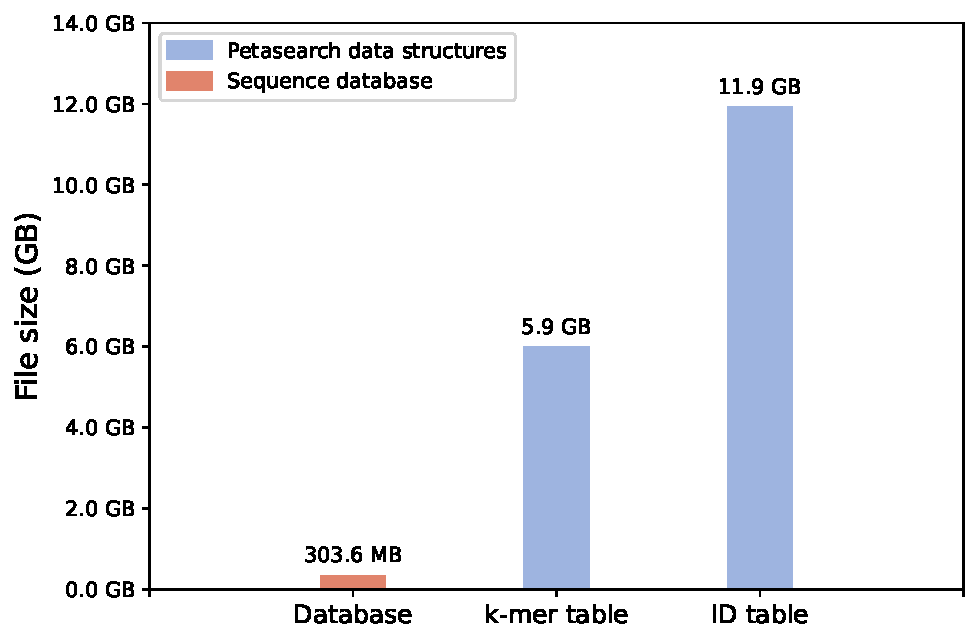
\includegraphics[width=.8\textwidth]{images/k11_space_consumption.pdf}
    \captionof{figure}{\textbf{Visualizaiton of k-mer table and ID table sizes when $\mathbf{k = 11}$.}
      The database is the \textit{UniProtKB/Swiss-Prot} database obtained through \texttt{mmseqs databases UniProtKB/Swiss-Prot swissprot tmp} command.
      Without optimization, the sizes of \texttt{petasearch} data structures are 6.46 times and 12.92 times larger than the sequence database.}
    \label{fig:k11_space}
  \end{figure}
  \begin{figure}
    \centering
    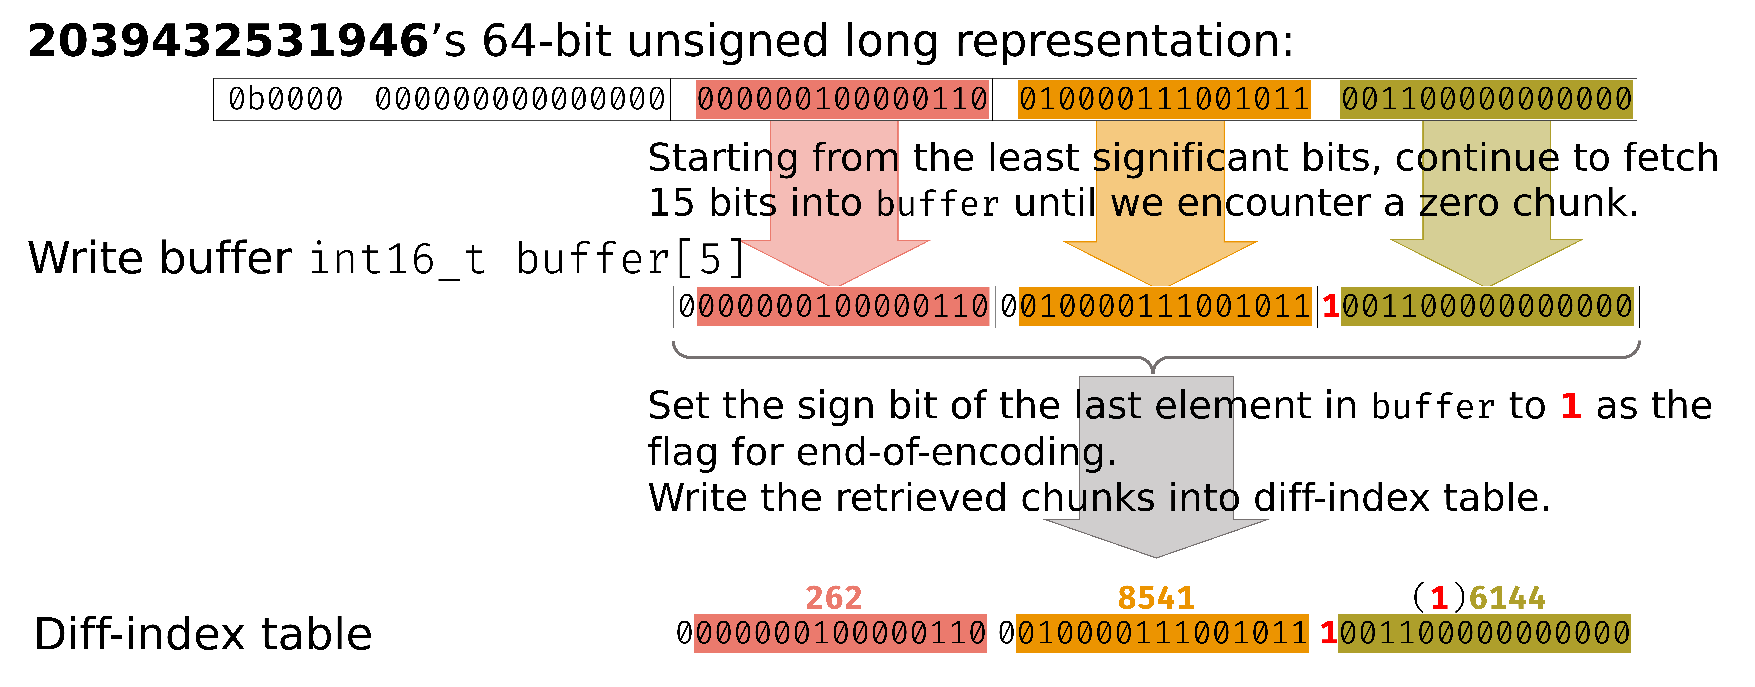
\includegraphics[width=\textwidth]{images/bit_squeezing_technique.pdf}
    \captionof{figure}{\textbf{The example decoding process of difference index $\mathbf{2039432531946}$.}
      We first retrieve 15-bit chunks starting from the least significant bits and store them into a write buffer in the reverse order until we encounter a zero chunk.
      For $2039432531946$, its highest non-zero bit is $39$, which means that we need three 16-bit \texttt{short} to store it.}
    \label{fig:bit_squeeze_technique}
  \end{figure}
\end{figpage}
\pagebreak

\subsection{IO Performance Optimization} \label{section:io-performance}

In the prototypical \texttt{Petasearch} implementation, \texttt{mmap} was selected for reading \texttt{Petasearch} data structures stored on NVMe SSDs.
However, \texttt{mmap} does not scale well with the increase in threads \cite{papagiannis2020optimizing} and thus cannot saturate the full throughput of NVMe SSDs.
To find the IO tool with the best performance, we conducted a benchmarking study on the performance of various IO tools using FIO benchmark software \cite{AxboeFlexibleIOTester2022}.
For synced IO tools, we benchmarked \texttt{pread} using different flags and \texttt{mmap}.
For async IO tools, we benchmarked \texttt{libaio} and \texttt{posix\_aio}.

The benchmarking results are visualized in \autoref{fig:fio_benchmark}.
It is clear that \texttt{libaio} performs the best.
I is able to saturate the full 3.5 GB/s linear read bandwidth of NVMe SSDs.
The other two tools, \texttt{posix\_aio} and \texttt{pread} with \texttt{O\_DIRECT} (\texttt{ioengine = psync} in FIO) have roughly the same performance, with bandwidth around 3.3 GB/s.
Unfortunately, \texttt{mmap} has the worst performance, with only about 1.5 GB/s at maximum.
The performance even fell to 0.25 GB/s when it scaled to 20 threads.
Since \texttt{mmap} is a synced IO module, adopting another synced IO module will require almost no change in control logic.
Considering both the performance and difficulty of refactoring, we chose to use \texttt{pread} with \texttt{O\_DIRECT} in place of \texttt{mmap}.

The implementation of \texttt{pread} with \texttt{O\_DIRECT} is rather simple: we simply create a read buffer according to the currently available memory size, open the k-mer diff-index file with \texttt{O\_DIRECT} flag, and then read in parallel using \texttt{pread} continuously untill \texttt{EOF} (end of file).

\subsection{Simplified Database Index} \label{section:simplified-database-index}

In \texttt{Petasearch} prototype, the sequence database format is the same as that of \texttt{MMseqs2}, which uses a complexed index structure for it having many functions.
Such complexity is unnecessary for \texttt{Petasearch}, especially when the database is huge in size, making the overhead for a complicated index become non-trivial.
Hence, we simplified the index, only preservingthe offset of the corresponding entry in the sequence database.
The simple yet efficient chagne not only reduce the IO overhead, but also derease the space consumption.

\subsection{Fast Third-Party Libraries}

We integrated several fast thrid-party libraries to replace the slow implementaions in \texttt{Petaserch} prototype.
The fast parallel in-place sorting algorithm $IPS^4o$ \cite{axtmann2017place} was integrated to replace the slow \texttt{std::sort}.
The banded Smith-Waterman-Gotoh aligner \texttt{block-aligner} \cite{liu2021block} was used to allow fast pairwise alignment in the third phase.

\pagebreak
\begin{figpage}
  \thispagestyle{fancy}
  \begin{figure}[htbp]
    \centering
    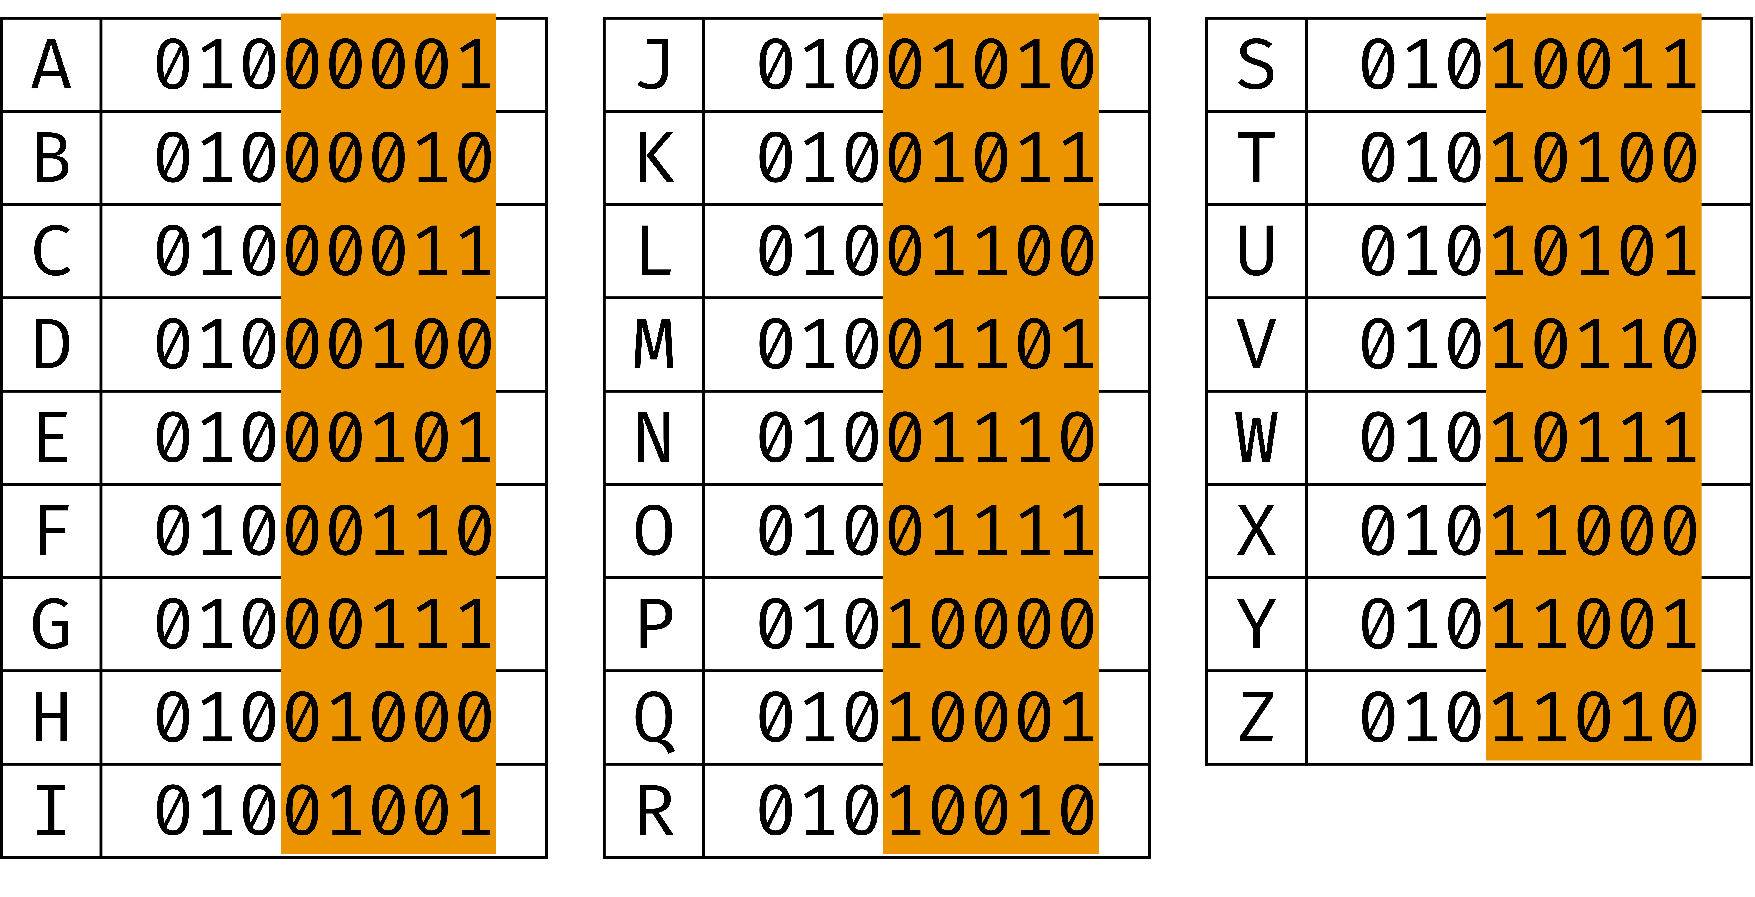
\includegraphics[width=.6\textwidth]{images/ASCII_prot.pdf}
    \caption{\textbf{Part of the ASCII table, showing the bit representation of \texttt{A} to \texttt{Z} with the last 5 bits highlighted.}
      It can be clearly seen that for \texttt{A} to \texttt{Z} in the English alphabet, we can represent them using only 5 bits instead of a whole byte (8 bits).}
    \label{fig:ascii_prot}
    \bigskip
    \begin{flushright}
      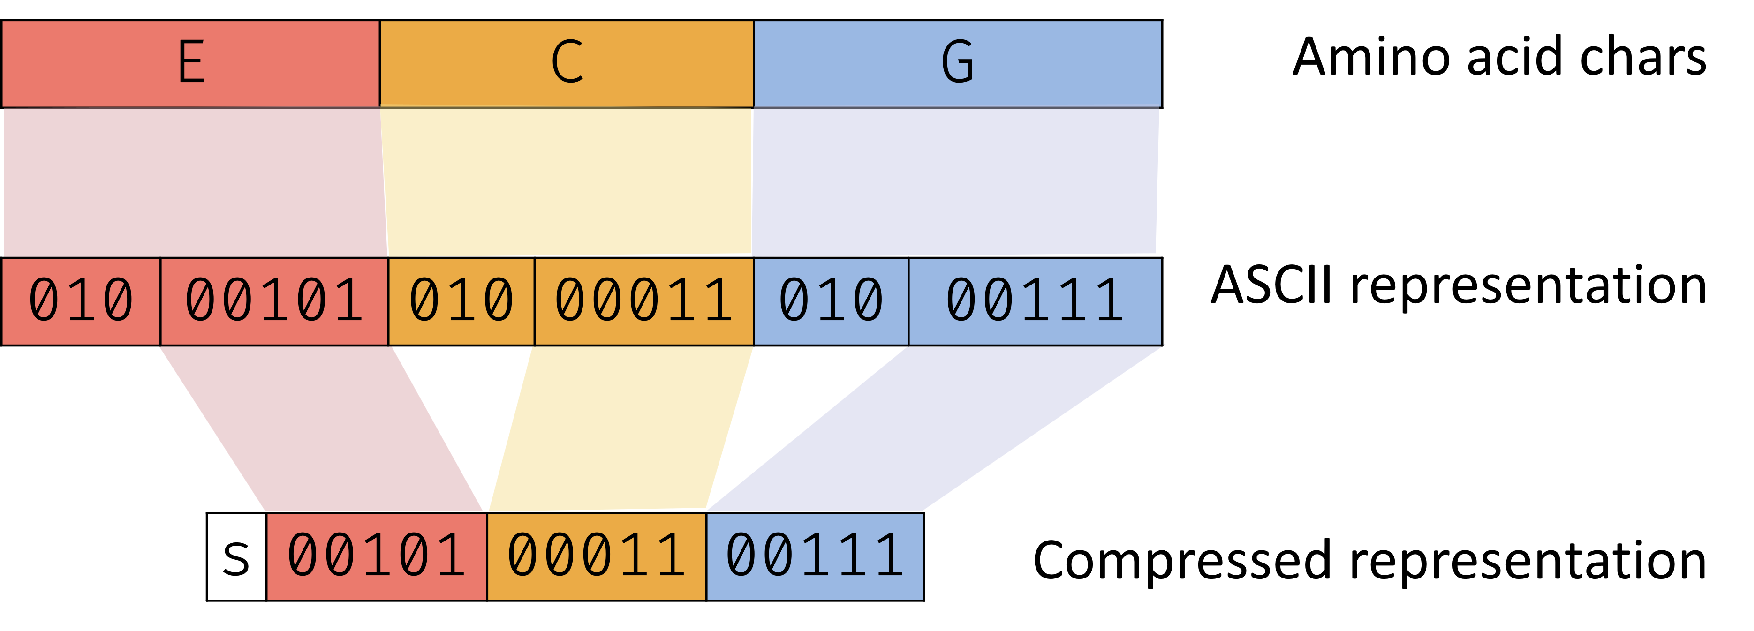
\includegraphics[width=.9\textwidth]{images/prot_seq_compress.pdf}
    \end{flushright}
    \caption{The example compression of short peptide glutathione (GSH).
      GSH consists of only three amino acids: glutamate (E), cysteine (C), and glycine (G).
      We simply fetch the least significant 5 bits of each amino acid \texttt{char} and store them into a single 16-bit \texttt{short}.}
    \label{fig:prot_seq_compress}
    \bigskip
    \centering
    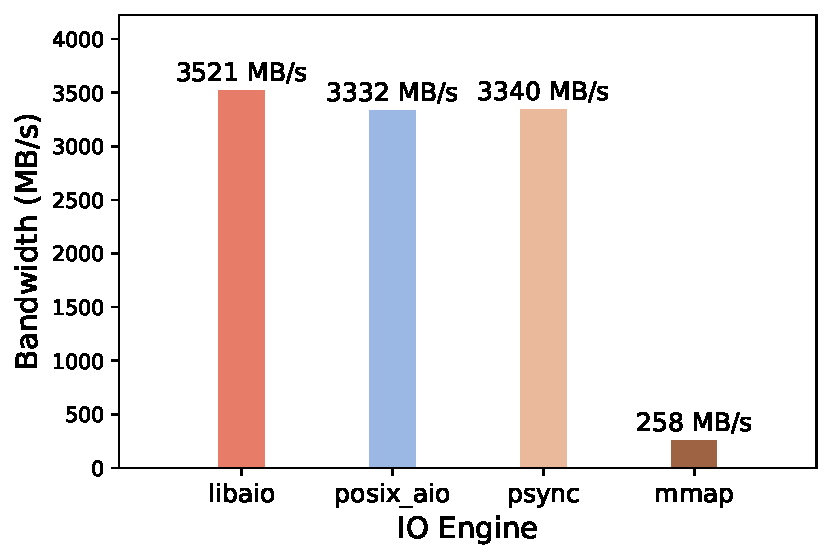
\includegraphics[width=.65\textwidth]{images/fio_benchmark.pdf}
    \caption{Benchmarking results of various IO tools using FIO benchmark software.
      The benchmark setting is imitating a parallel read from 20 NVMe SSDs.
      A total of 20 threads were created, each one responsible of reading a 50 GB file stored on one NVMe SSD.
      The bandwidth is the average reading bandwidth per SSD.
      The IO engine \texttt{psync} is equivalent to opening a file handle with \texttt{O\_DIRECT} and reading from the handle using \texttt{pread}.}
    \label{fig:fio_benchmark}
  \end{figure}
\end{figpage}
\pagebreak

\section{Sensitivity Improvement} \label{section:sensitivity-improvement}

The k-mer matching mechanism limits \texttt{Petasearch}'s ability of finding homologs for low sequence identity.
To improve \texttt{Petasearch}'s performance at lower sequence identity, we made \texttt{Petasearch} able to perform profile search by allowing profile databases as inputs.

Profile search is using a "sequence profile" generated from multiple sequence alignment (MSA) results as the querying input \cite{steinegger2019hh}.
The profile Hidden Markov Model (HMM) provides position-specific aminoaid insertion, deleletion and substitution penalties \cite{steinegger2019hh}, which significantly increase the searching sensitivity.
The most sensitive searching tools such as \texttt{HMMER} \cite{eddy2009new}, \cite{eddy2011accelerated}, \texttt{HHblits} \cite{remmert2012hhblits} and \texttt{HH-suite3} \cite{steinegger2019hh} all use the profile search mechanism.
Thus, enabling \texttt{Petasearch} to perform profile search is expected to improve its sensitivity at low sequence identity.

\section{Benchmarks} \label{section:benchmarks}

Since \texttt{Petasearch} has been much improved and new features were also added, we also devised updated benchmarks to evaluate both the its speed and sensitivity.
We performed all the benchmarks on a server with AMD EPYC 7702P (128) @ 2.000GHz CPUs, 995 GB RAM, Debian GNU/Linux 11, twenty two Samsung 970 EVO Plus NVMe SSDs (2 TB) connected via PCI-Express.

\subsection{Speed Benchmark} \label{section:speed-benchmark}

In the time benchmark we measured the time that \texttt{Petasearch}, fast \texttt{MMseqs2} search with default parameters and \texttt{DIAMOND} search with both query-index mode (fast) and double-index mode (default) to search a small query set of 2.9 MB against a 9.3 TB large target set.
\texttt{Petasearch} was only conducted using 9-mers due to space limitation.
We used the original 456 GB data of Soil Reference Catalog (SRC) and Marine Eukaryotic Reference Catalog (MERC) \cite{steinegger2019plass} and duplicated several copies of them until we filled twenty NVMe disks fully with the sequence databases and \texttt{Petasearch} tables.
As a result, each NVMe roughly contains seven to eight 70GB databases.
We ran \texttt{Petasearch} algorithm ten times and
report the average run-time to avoid deviations.
The other two algorithms, due to their slowliness, were only run once to show the rough runtime magnitude.
We only varied the \texttt{--exact-k-mer-matching} parameter to control the creation of similar k-mers for \texttt{Petasearch}, and the \texttt{--algo} parameter for \texttt{DIAMOND} to choose between only indexing query and double-indexing.
All other parameters were set to default.

\subsection{Sensitivity Benchmark} \label{section:sensitivity-benchmark}

For the sensitivity benchmark we measured and compared the results of the \texttt{Petasearch} algorithm using both sequence search mode and profile search mode against \texttt{MMseqs2} sequence search (fast preset, \texttt{-s 5.7}), \texttt{MMseqs2} profile search (fast preset) and \texttt{DIAMOND} (fast and sensitive presets).
The main goal of this benchmark is to show that \texttt{Petasearch} is able to compete with the other, more sensitive algorithms in the upper sequence identity buckets, and the newly added profile search is able to have better sensitivity in the lower sequence identity buckets.

We downloaded the \textit{UniProt} database and randomly extracted one million entries and clustered them to $0.9$, $0.8$, $0.7$, $0.6$, $0.5$ and $0.4$ percent sequence identity using \texttt{MMseqs2}'s clustering workflow.
For each cluster, we randomly selected 5\% of the sequences as query database, and the remaining 95\% as target database.
For each sequence in every databases, we tagged the sequence with its domain information by using \texttt{MMseqs2} to search the "scop25 dbset" described by Hauser et.
al.
\cite{hauserbioinformaticsbtw006} against both query database and target database.
The sequence without any SCOP domain was filtered out.
For all other sequences in the query databases, we reversed the region that is not the SCOP25 domain; for target sequences, we shuffled those regions randomly.
In this way, we can use the domain information to identify false positive hits.
If the hits happen between two sequences with SCOP domain similarity lower than family level, we will consider it as false positive (FP).
Otherwise, it will be considered as true positive (TP).
For each algorithm, we only considered the best hit found for each query.
Since all algorithms
sort their hits by the E-value, we selected the hit with the highest E-value.
